\subsubsection{MPC3 - Indice Gulpease}
Di seguito è riportato il grafico dell'indice di Gulpease calcolato sui vari documenti, il cui valore è definito accettabile e ottimale come descritto nella sezione §2.2.1.1.\\

\myparagraph{Grafico complessivo}

\begin{figure}[H]
\centering
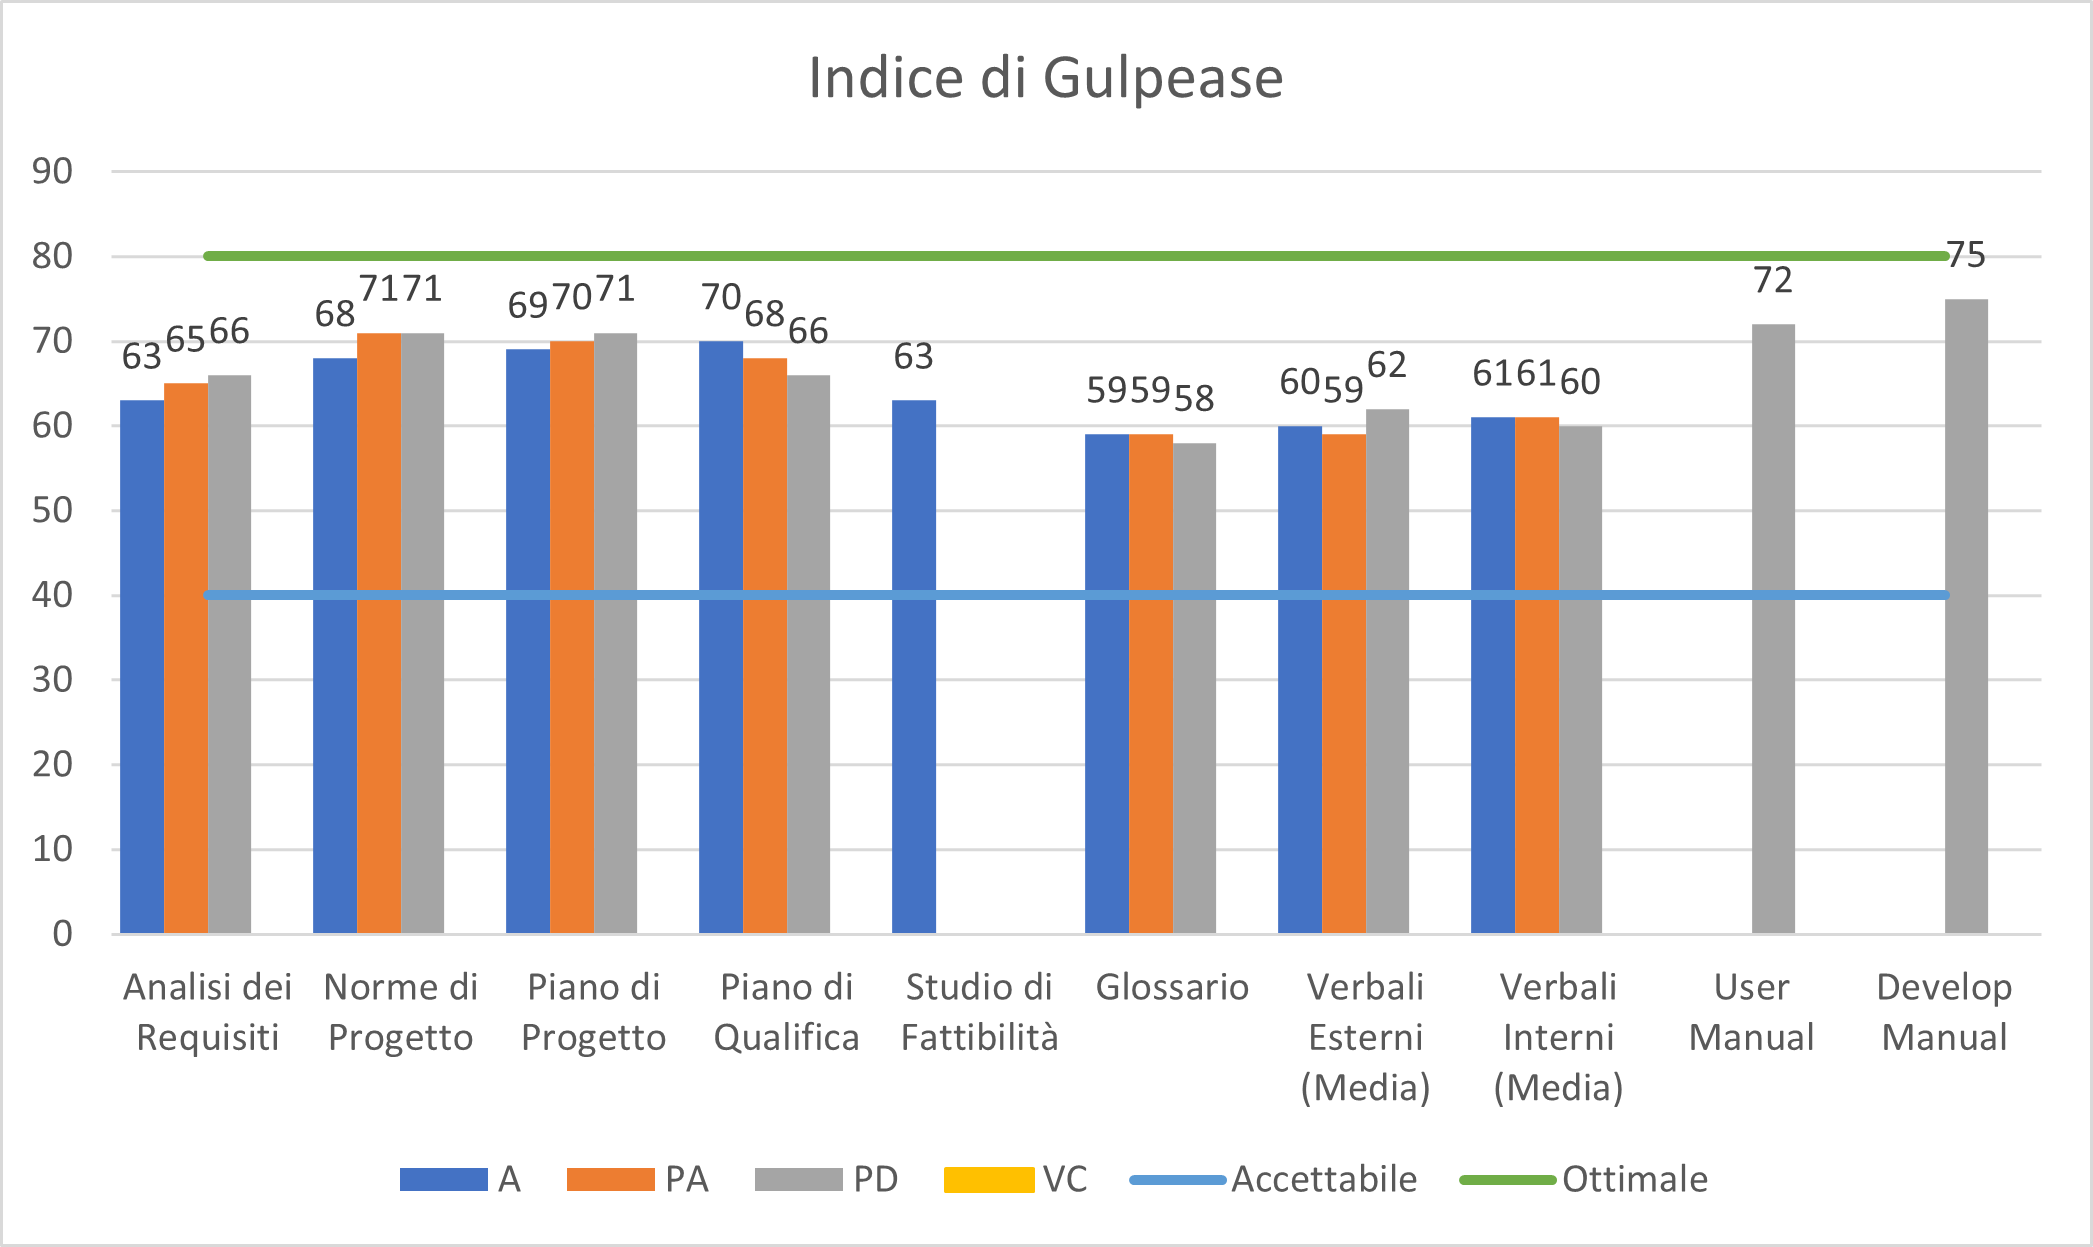
\includegraphics[scale=0.78]{res/ResocontoAttivitaDiVerifica/res/metriche/grafici/img/indiceGulpease.png}\\
\caption{Andamento complessivo dell'indice di Gulpease}
\end{figure}


\myparagraph{Grafico per documento}
\begin{figure}[H]
\centering
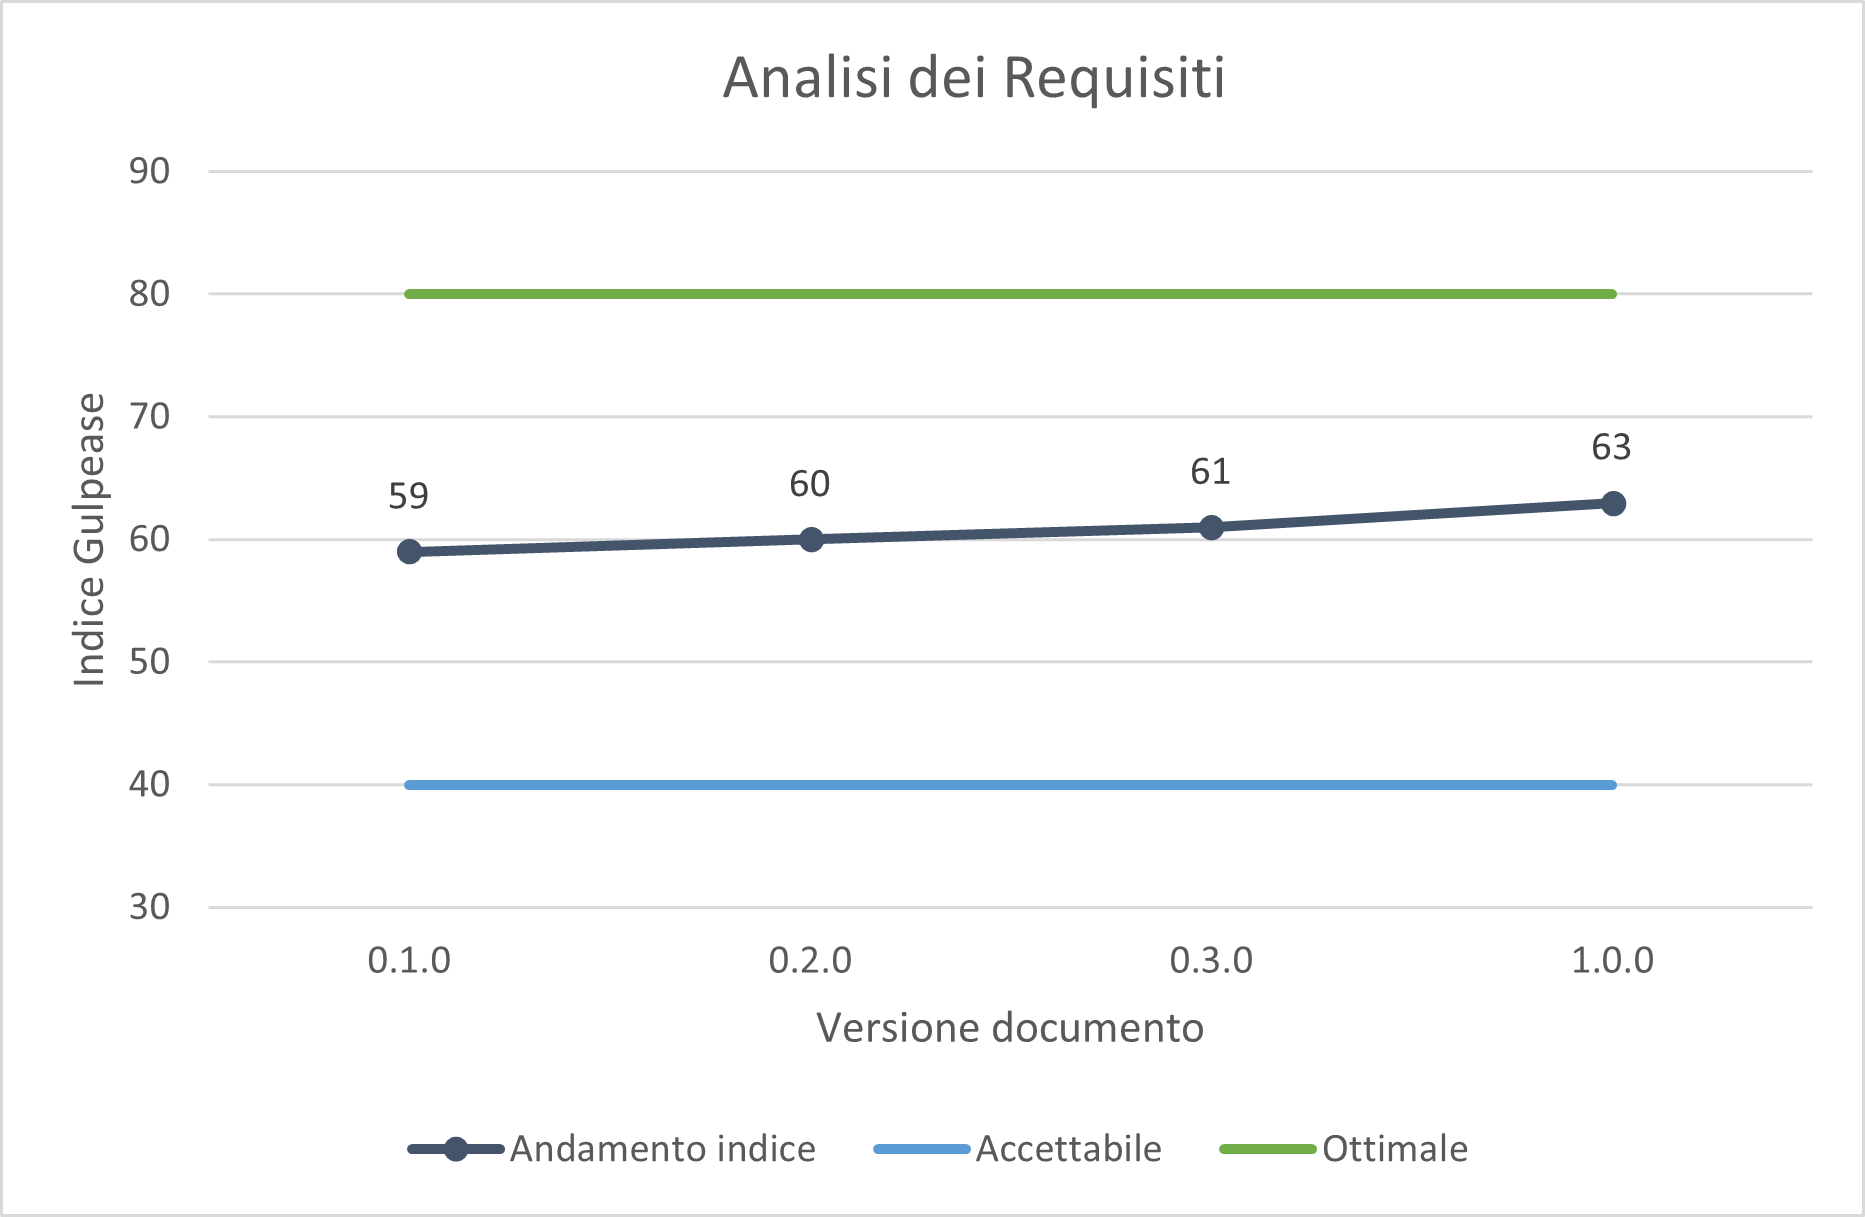
\includegraphics[scale=0.78]{res/ResocontoAttivitaDiVerifica/res/metriche/grafici/img/gulpeaseADR.png}\\
\caption{Andamento dell'indice di Gulpease \AdR}
\end{figure}

\begin{figure}[H]
\centering
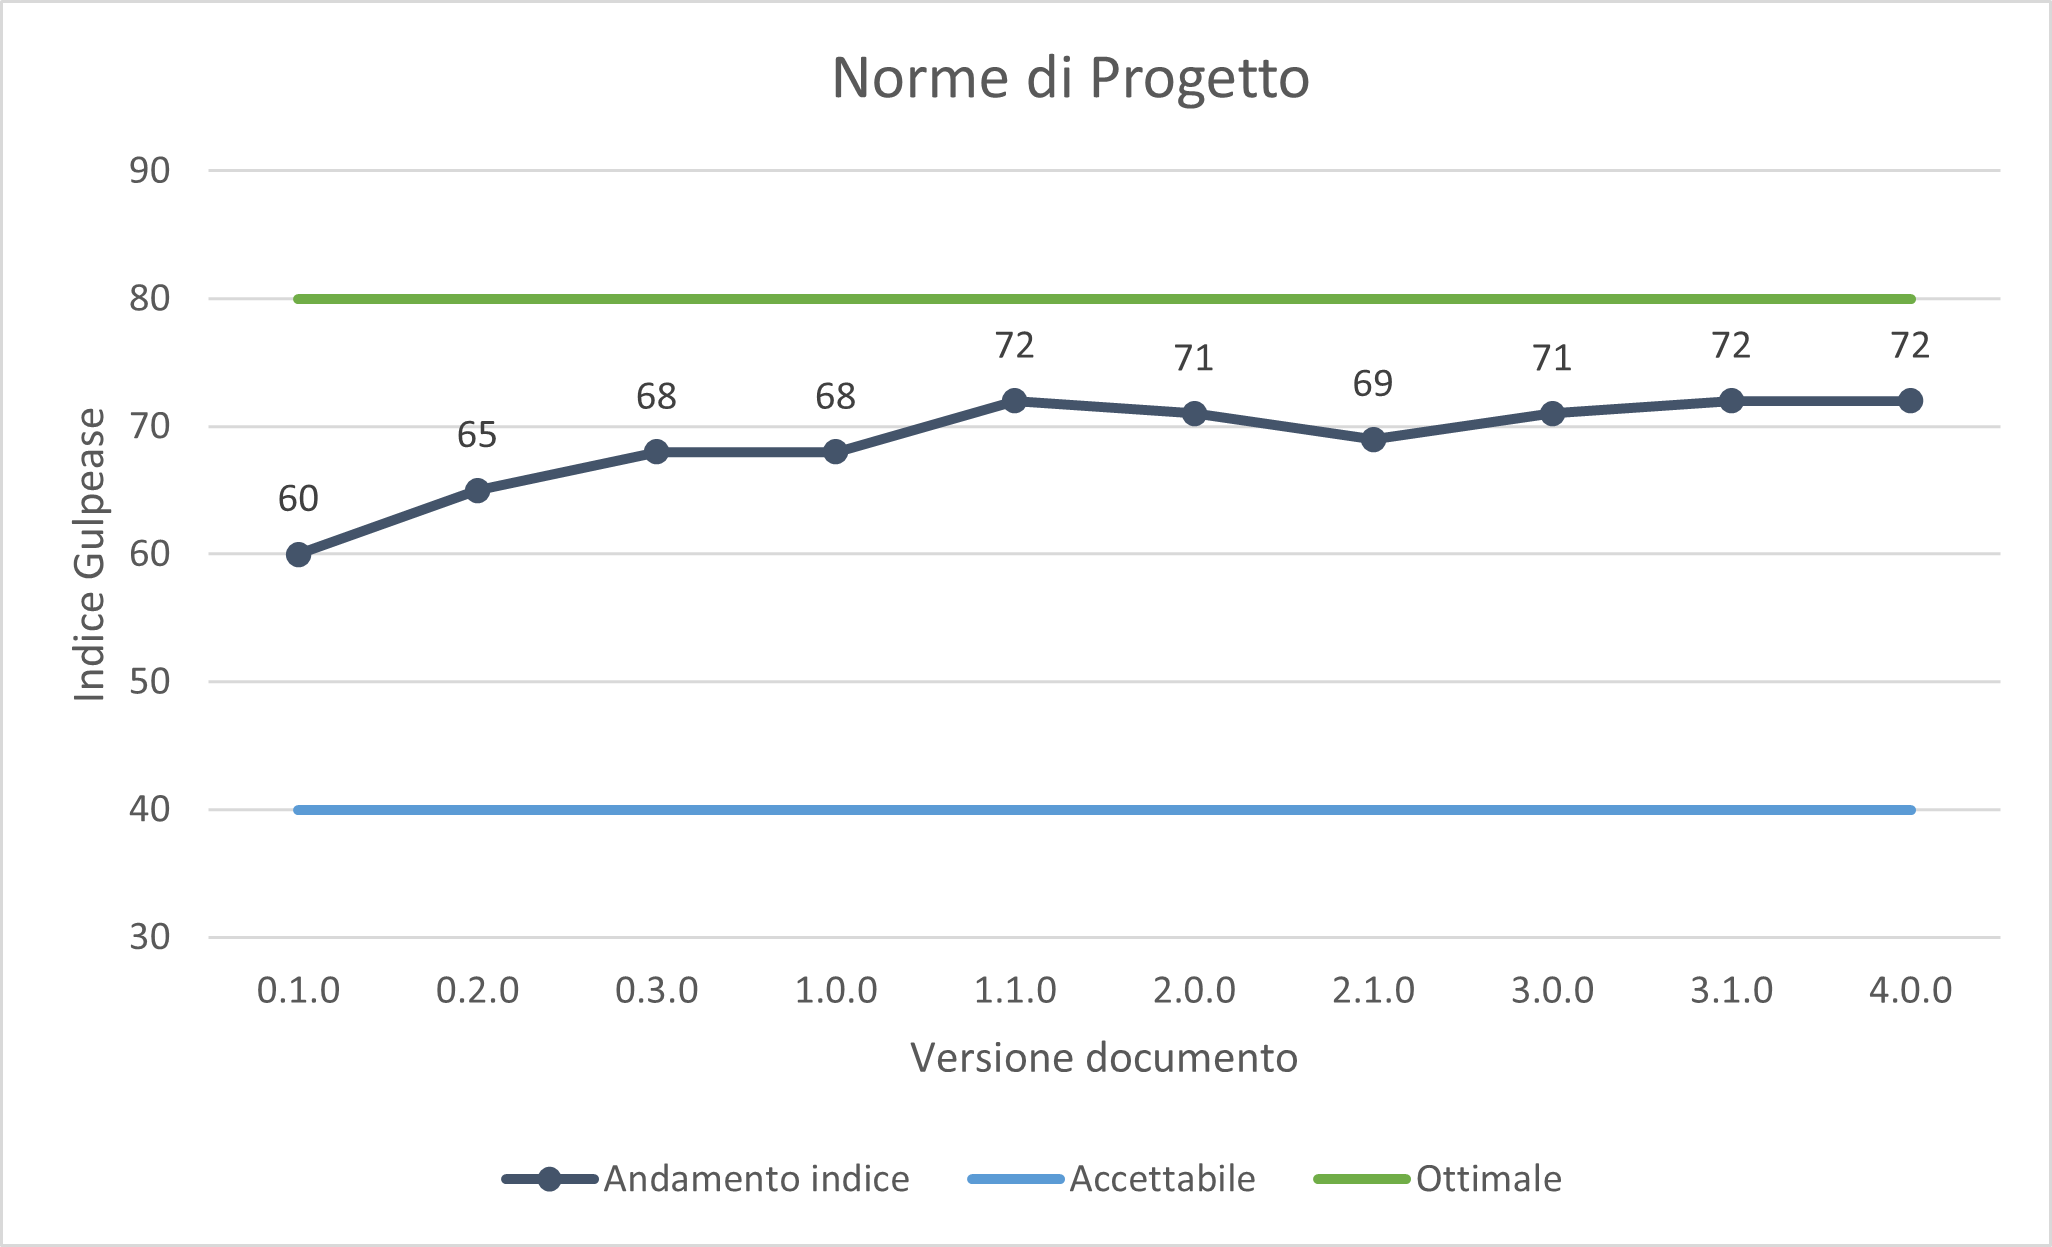
\includegraphics[scale=0.78]{res/ResocontoAttivitaDiVerifica/res/metriche/grafici/img/gulpeaseNDP.png}\\
\caption{Andamento dell'indice di Gulpease \NdP}
\end{figure}

\begin{figure}[H]
\centering
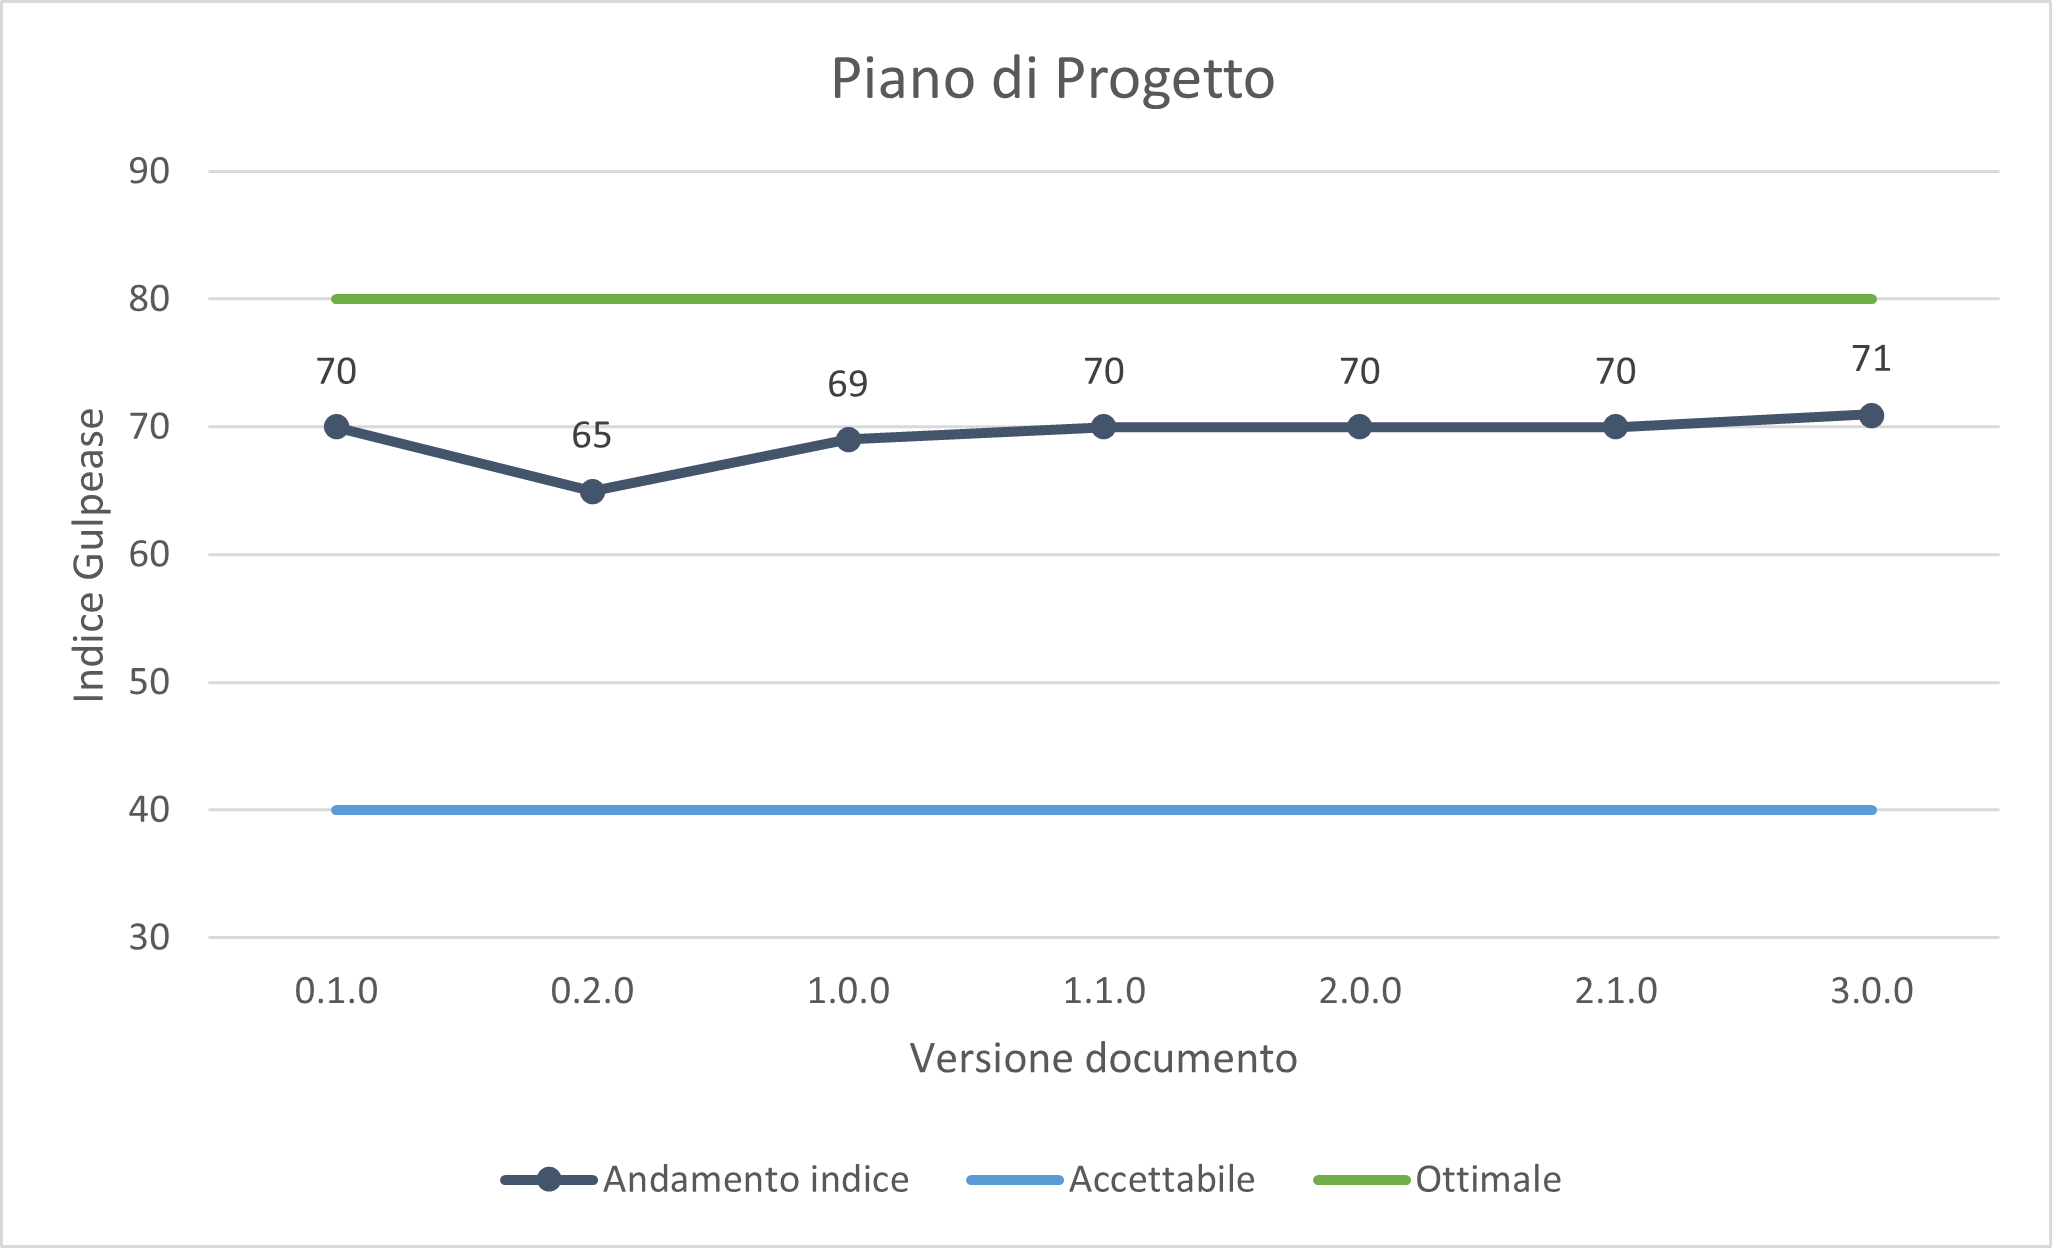
\includegraphics[scale=0.78]{res/ResocontoAttivitaDiVerifica/res/metriche/grafici/img/gulpeasePDP.png}\\
\caption{Andamento dell'indice di Gulpease \PdP}
\end{figure}

\begin{figure}[H]
\centering
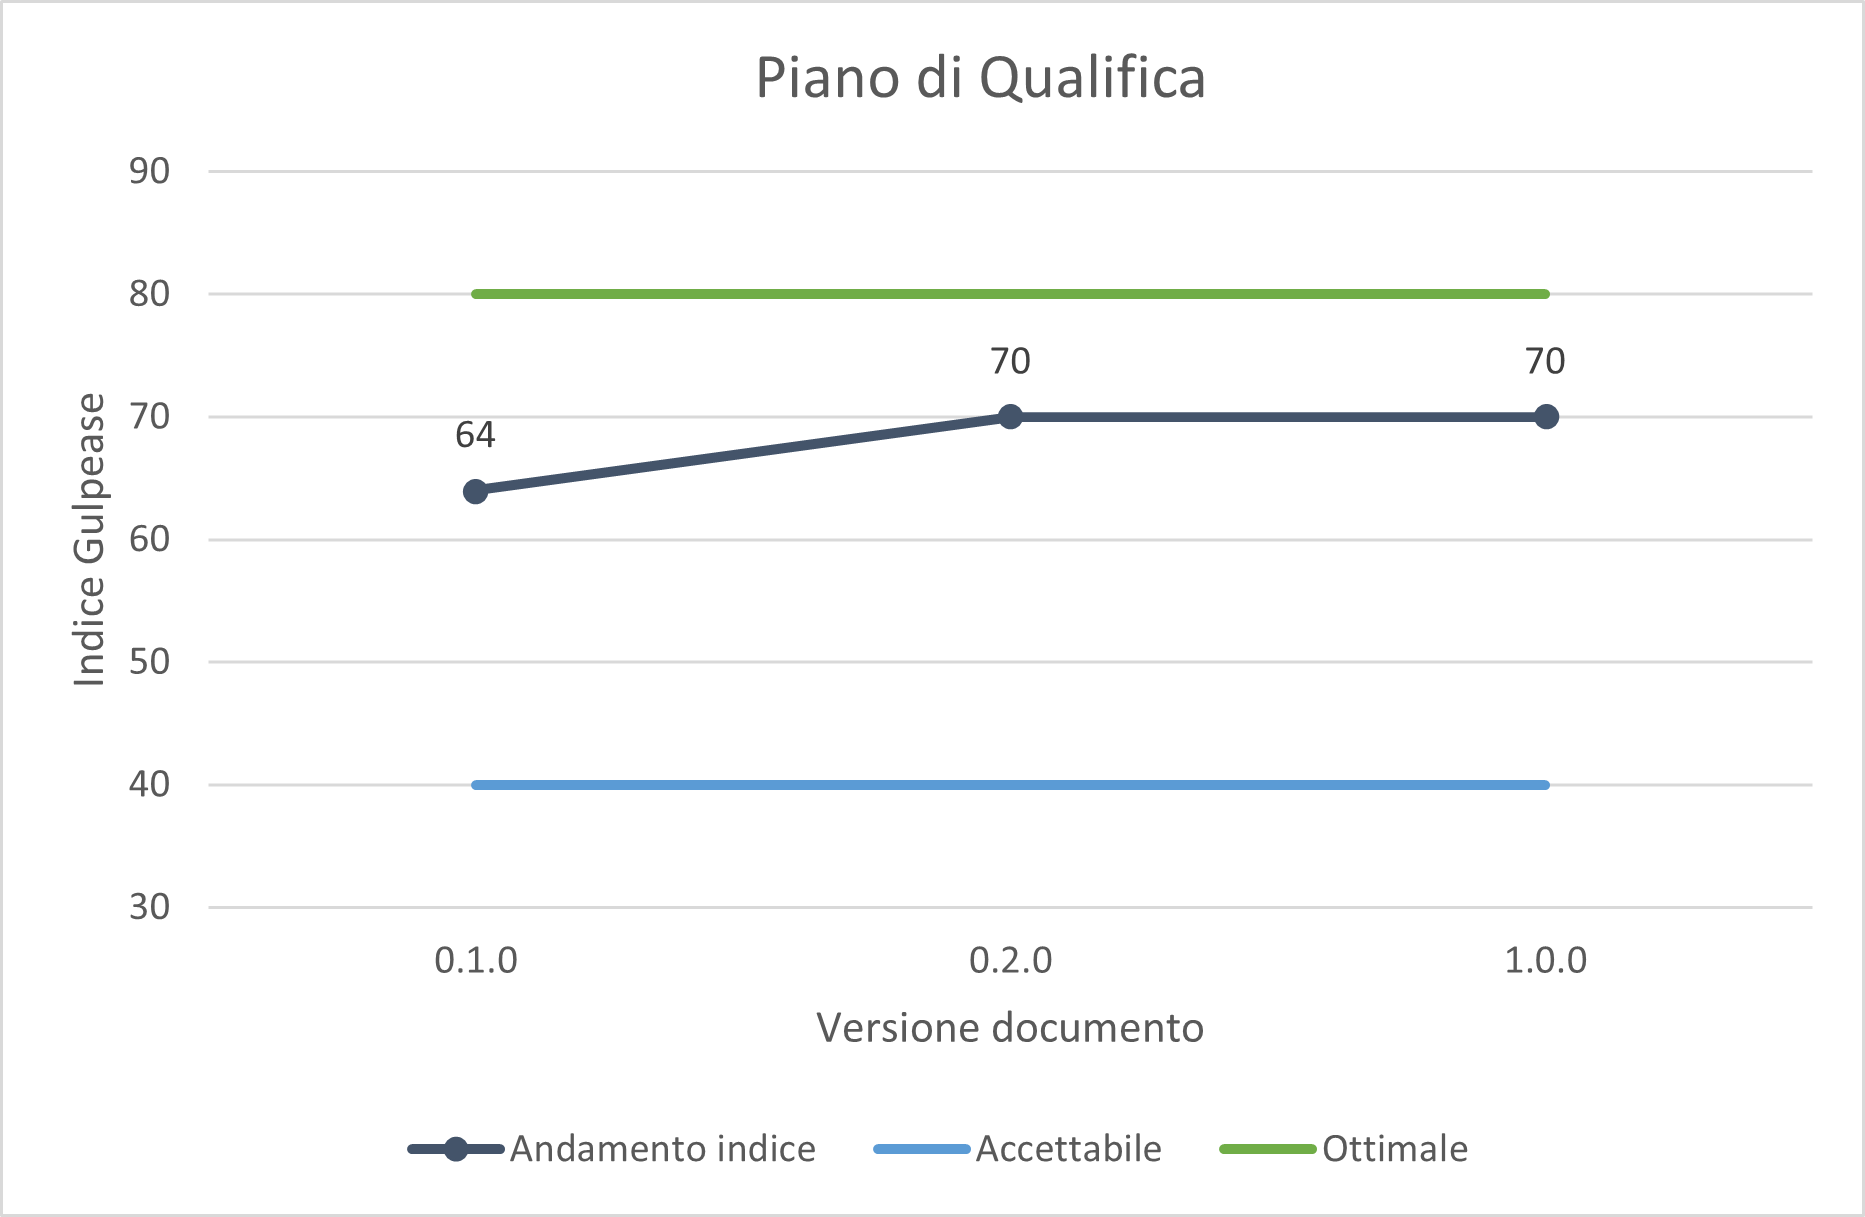
\includegraphics[scale=0.78]{res/ResocontoAttivitaDiVerifica/res/metriche/grafici/img/gulpeasePDQ.png}\\
\caption{Andamento dell'indice di Gulpease \PdQ}
\end{figure}

\begin{figure}[H]
\centering
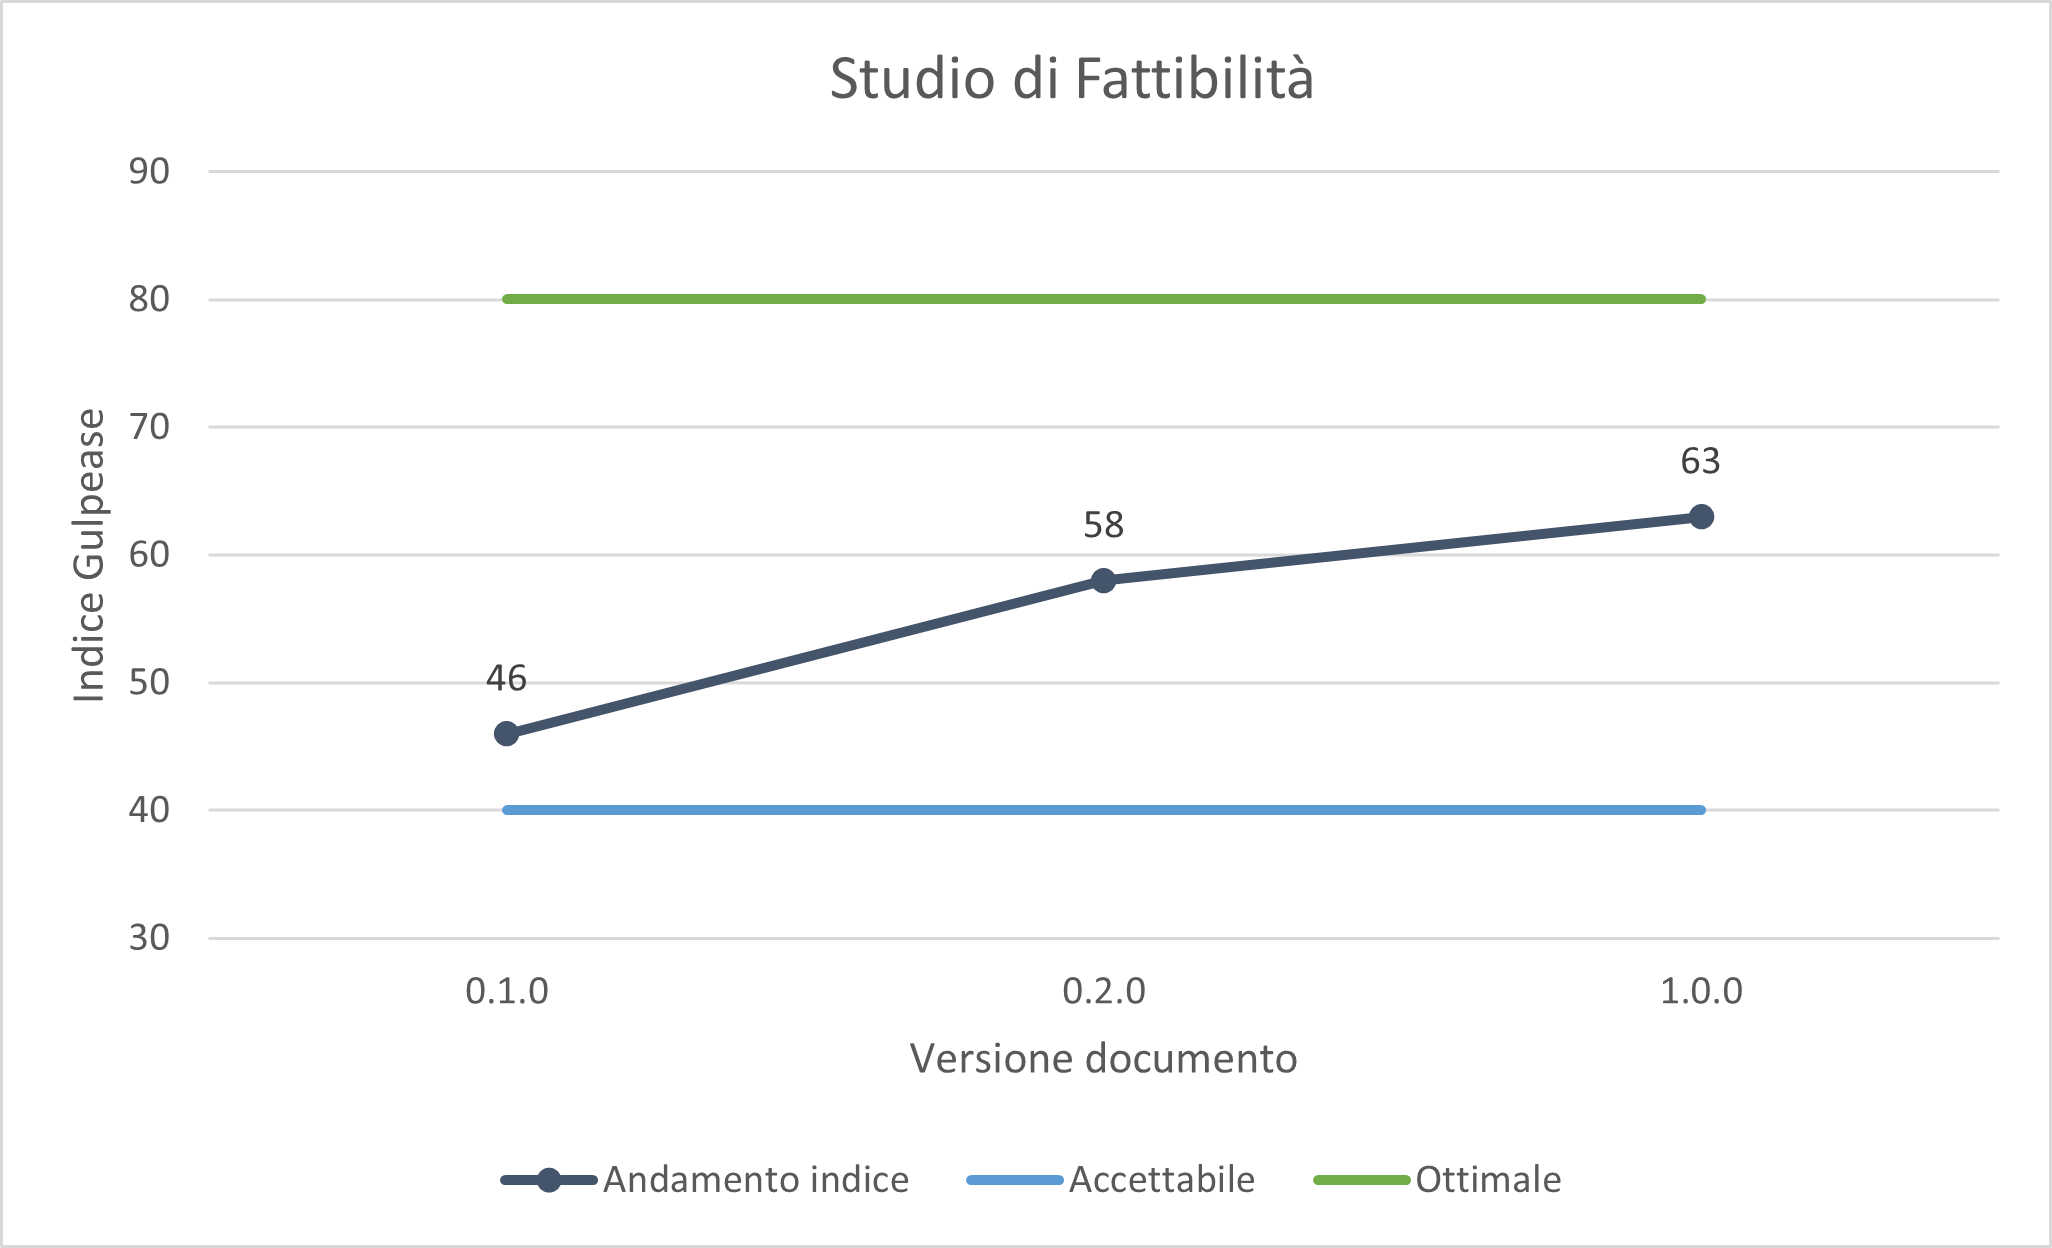
\includegraphics[scale=0.78]{res/ResocontoAttivitaDiVerifica/res/metriche/grafici/img/gulpeaseSDF.png}\\
\caption{Andamento dell'indice di Gulpease \SdF}
\end{figure}

\begin{figure}[H]
\centering
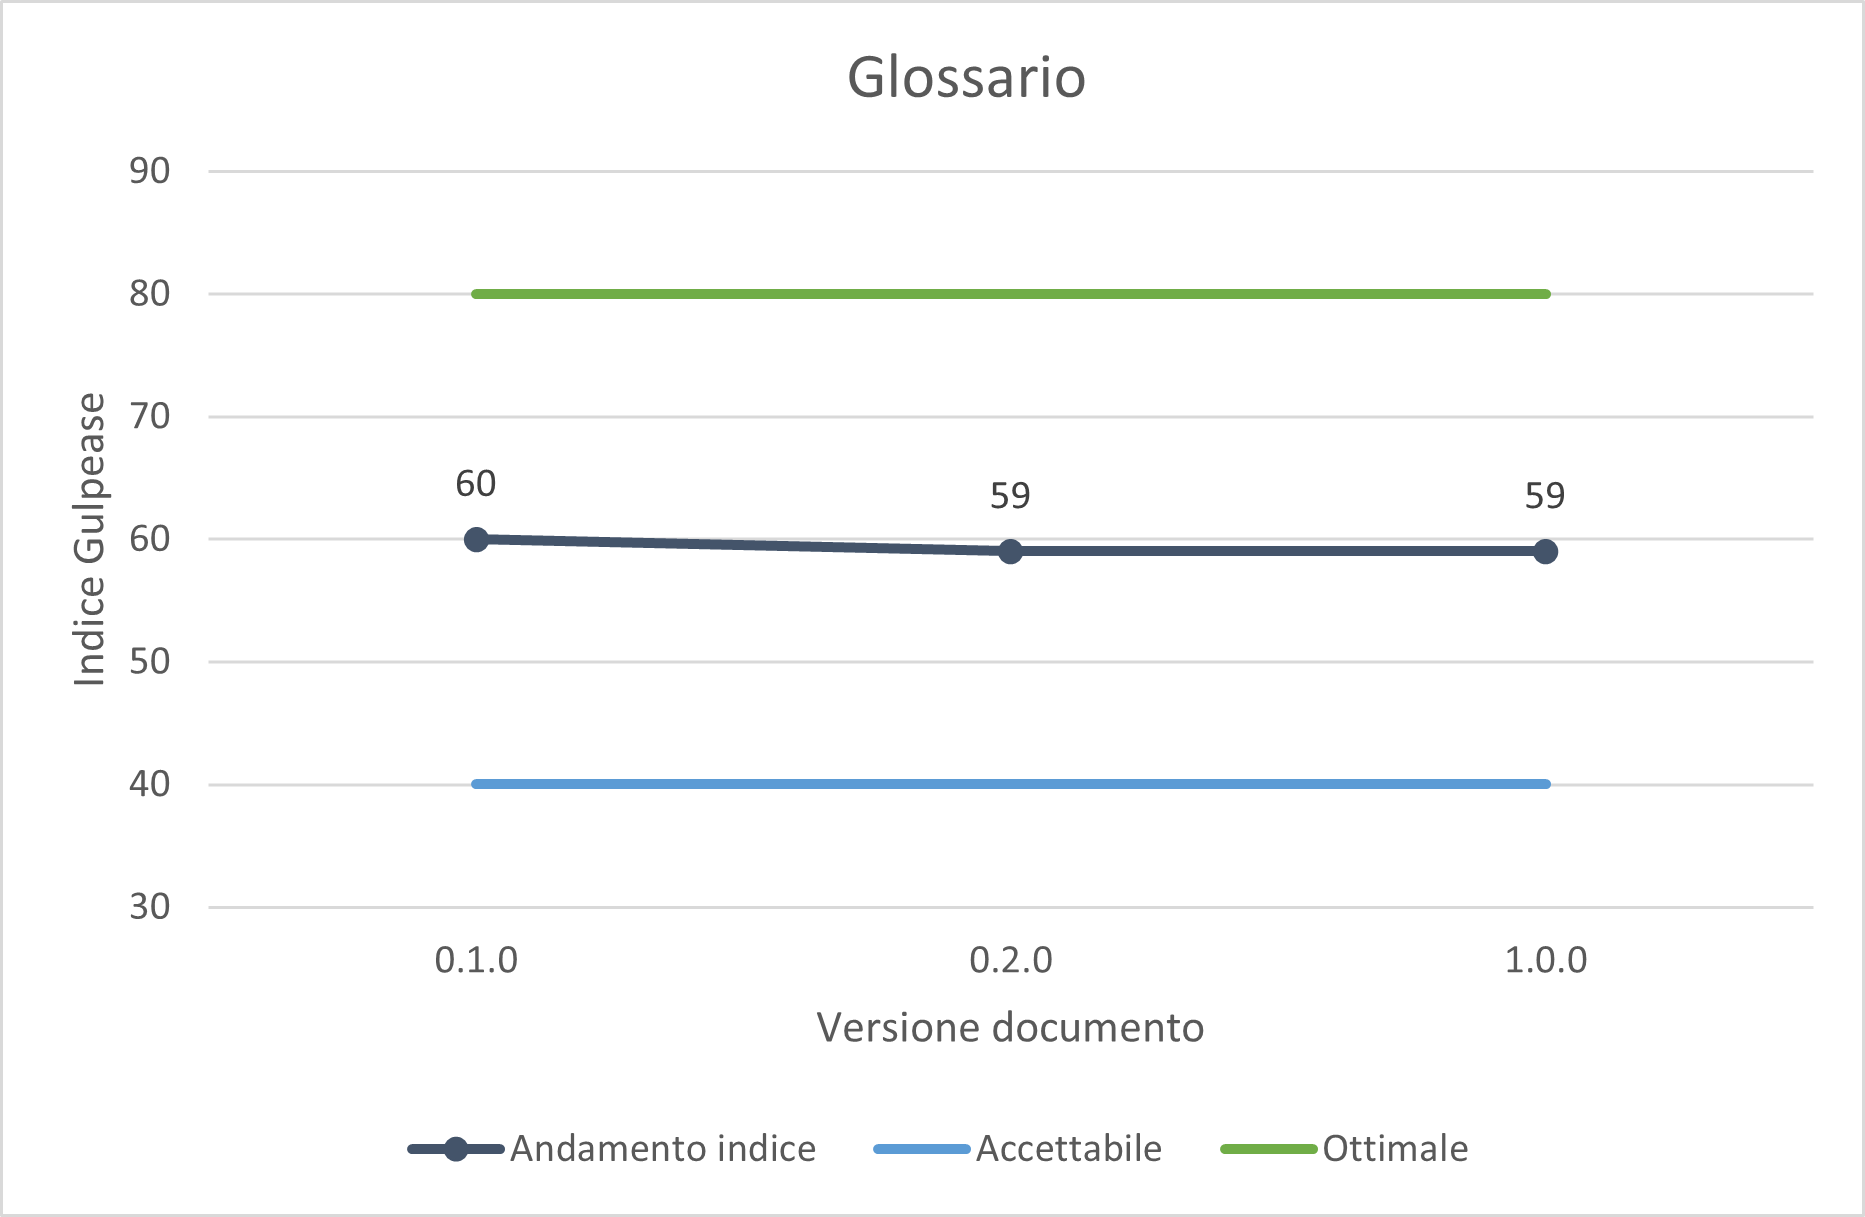
\includegraphics[scale=0.78]{res/ResocontoAttivitaDiVerifica/res/metriche/grafici/img/gulpeaseG.png}\\
\caption{Andamento dell'indice di Gulpease \Glossario}
\end{figure}

\begin{figure}[H]
\centering
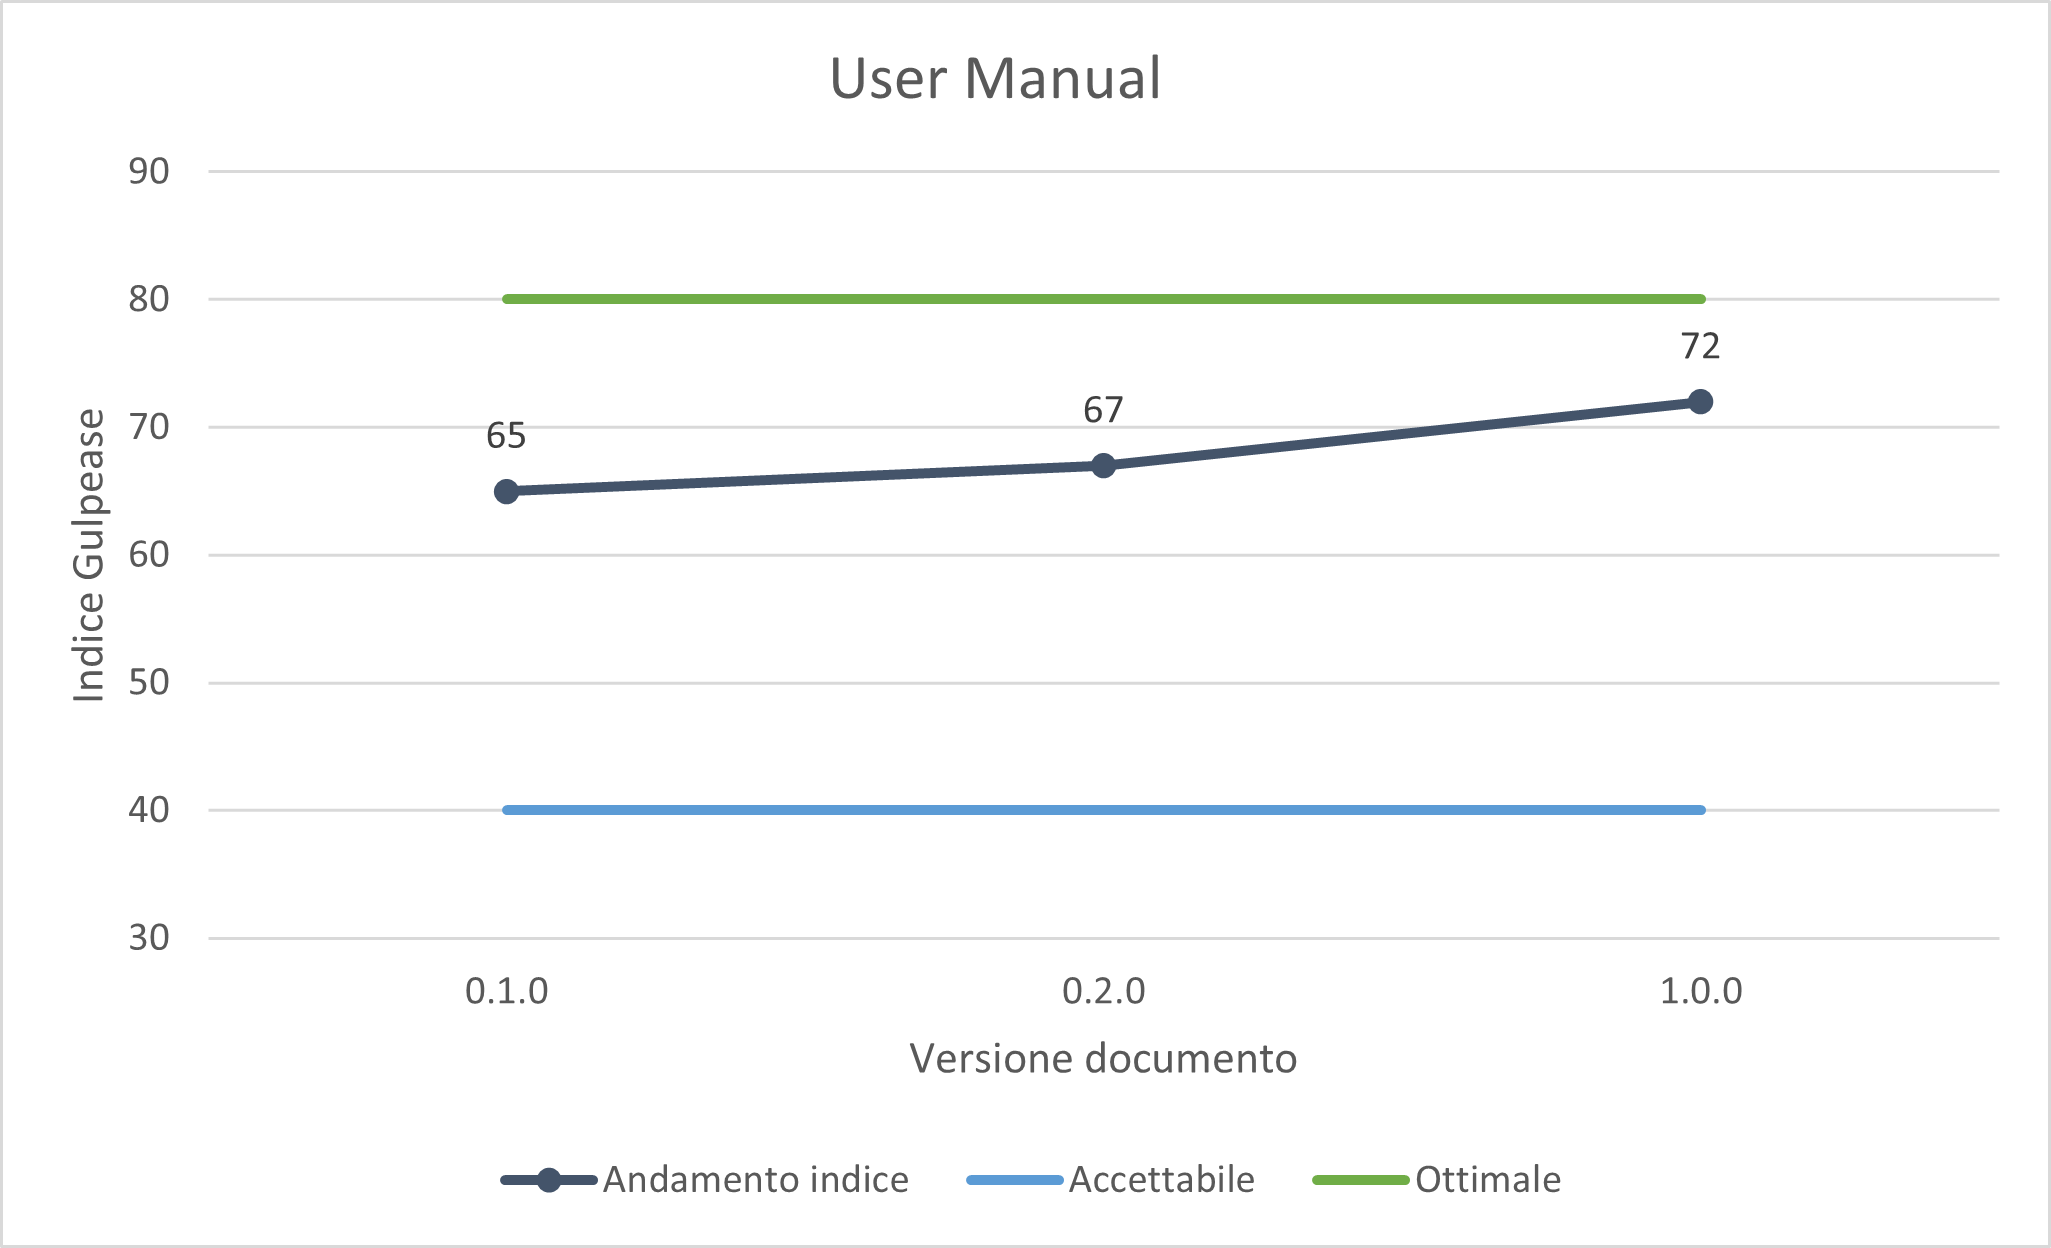
\includegraphics[scale=0.78]{res/ResocontoAttivitaDiVerifica/res/metriche/grafici/img/gulpeaseUM.png}\\
\caption{Andamento dell'indice di Gulpease \MU}
\end{figure}

\begin{figure}[H]
\centering
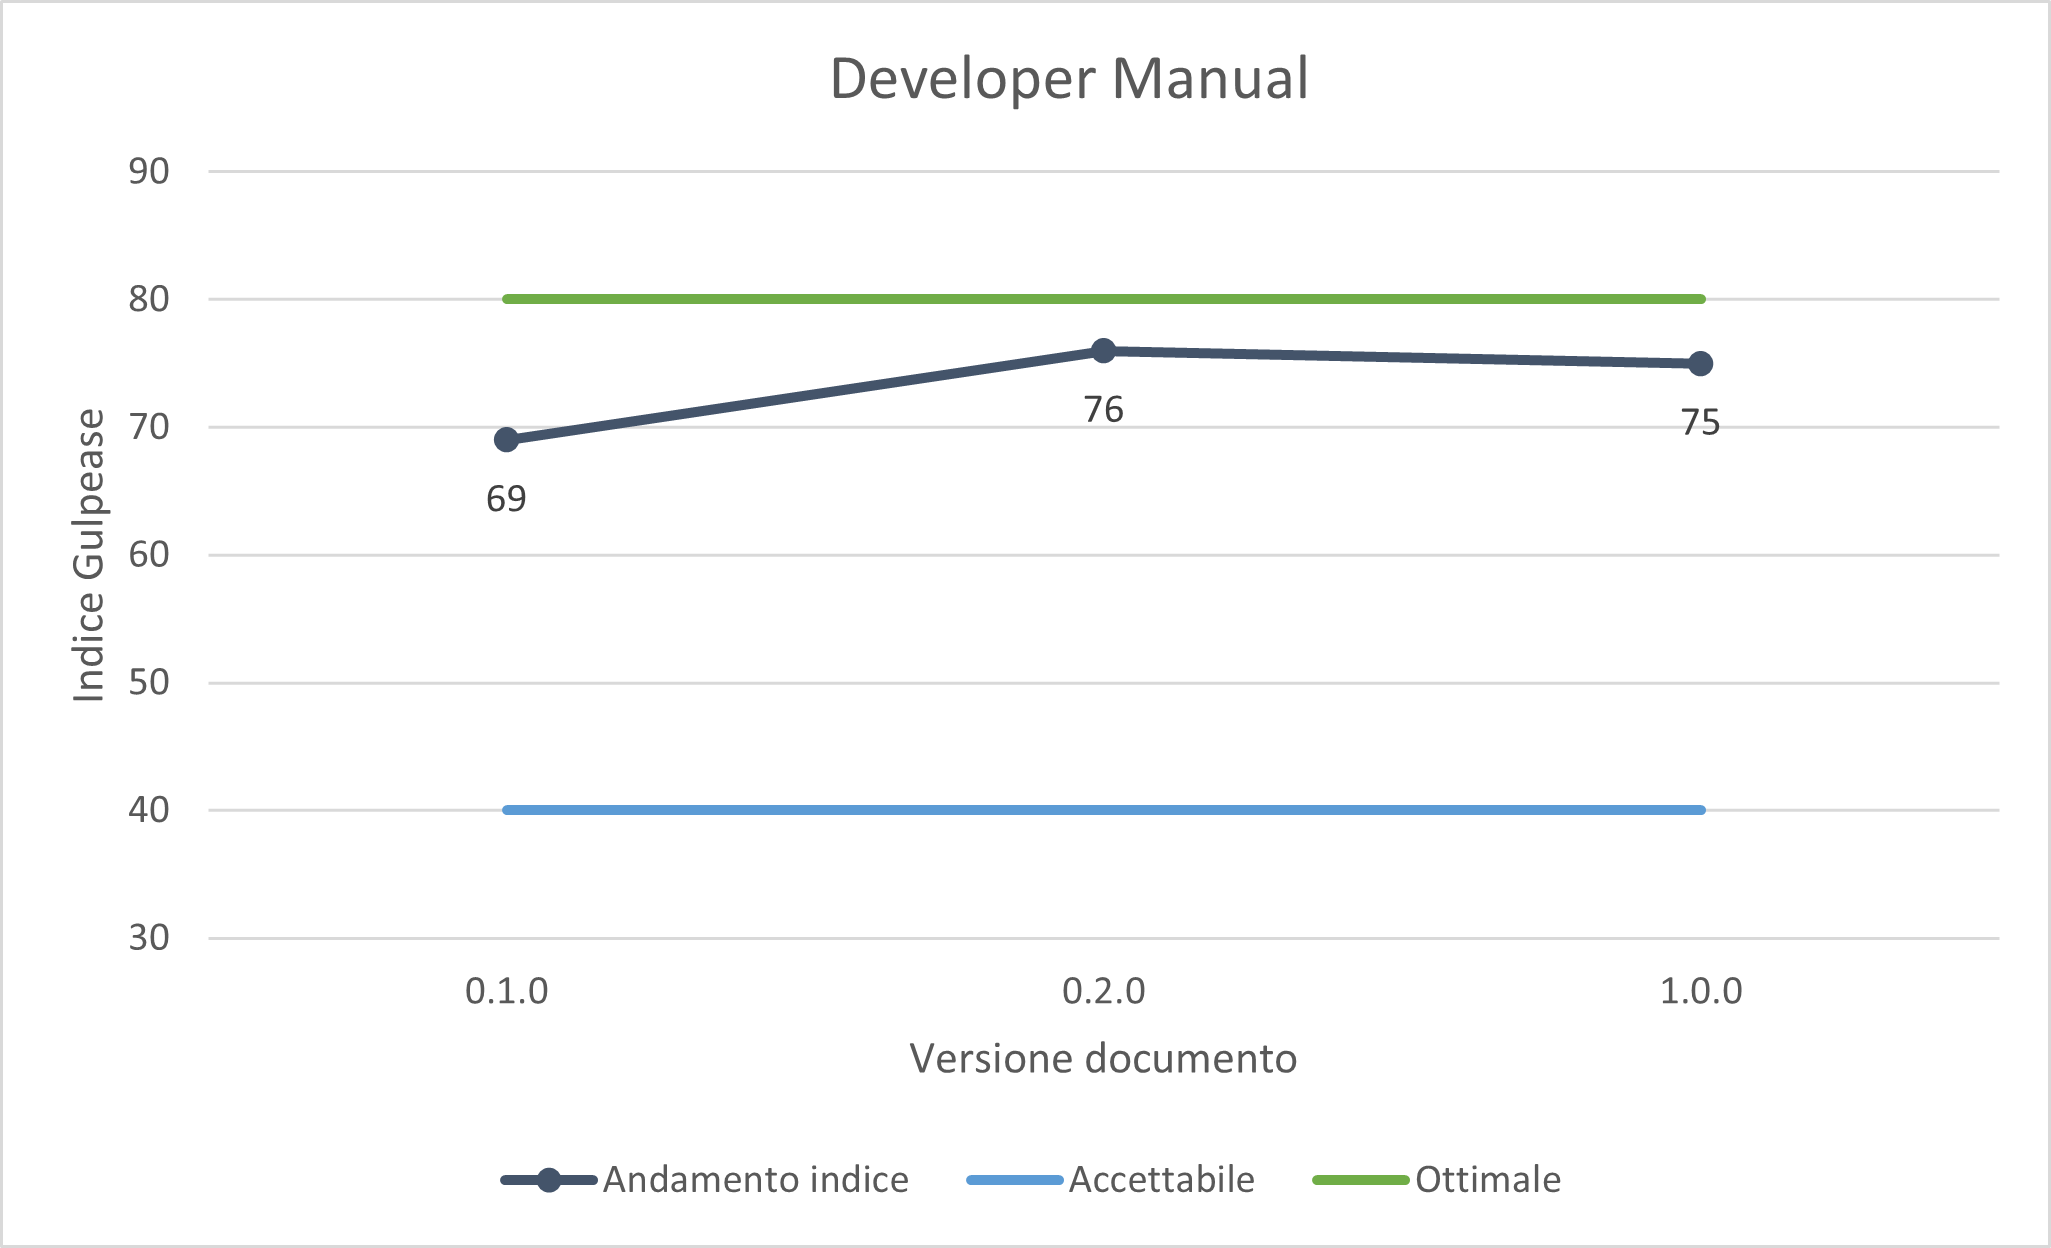
\includegraphics[scale=0.78]{res/ResocontoAttivitaDiVerifica/res/metriche/grafici/img/gulpeaseDM.png}\\
\caption{Andamento dell'indice di Gulpease \MM}
\end{figure}

